%%%%%%%%%%%%%%%%%%%%%%% file template.tex %%%%%%%%%%%%%%%%%%%%%%%%%
%
% This is a general template file for the LaTeX package SVJour3
% for Springer journals.          Springer Heidelberg 2010/09/16
%
% Copy it to a new file with a new name and use it as the basis
% for your article. Delete % signs as needed.
%
% This template includes a few options for different layouts and
% content for various journals. Please consult a previous issue of
% your journal as needed.
%
%%%%%%%%%%%%%%%%%%%%%%%%%%%%%%%%%%%%%%%%%%%%%%%%%%%%%%%%%%%%%%%%%%%
%
% First comes an example EPS file -- just ignore it and
% proceed on the \documentclass line
% your LaTeX will extract the file if required
\begin{filecontents*}{example.eps}
%!PS-Adobe-3.0 EPSF-3.0
%%BoundingBox: 19 19 221 221
%%CreationDate: Mon Sep 29 1997
%%Creator: programmed by hand (JK)
%%EndComments
gsave
newpath
  20 20 moveto
  20 220 lineto
  220 220 lineto
  220 20 lineto
closepath
2 setlinewidth
gsave
  .4 setgray fill
grestore
stroke
grestore
\end{filecontents*}
%
\RequirePackage{fix-cm}
%
%\documentclass{svjour3}                     % onecolumn (standard format)
%\documentclass[smallcondensed]{svjour3}     % onecolumn (ditto)
%\documentclass[smallextended]{svjour3}       % onecolumn (second format)
\documentclass[twocolumn]{svjour3}          % twocolumn
%
\smartqed  % flush right qed marks, e.g. at end of proof
%
\usepackage{graphicx}    %figuras
\usepackage[utf8]{inputenc} %tildes 
\usepackage{multirow,array}  %tablas
\usepackage{float}      %Posicion de las figuras H
%
% \usepackage{mathptmx}      % use Times fonts if available on your TeX system
%
% insert here the call for the packages your document requires
%\usepackage{latexsym}
% etc.
%
% please place your own definitions here and don't use \def but
% \newcommand{}{}
%
% Insert the name of "your journal" with
% \journalname{paper_wtb}


\begin{document}

\title{STRUCTURAL DESIGN OF CARBON/EPOXY BIOINSPIRED WIND TURBINE BLADE USING FLUID/STRUCTURE SIMULATION%Insert your title here%\thanks{Grants or other notes
%about the article that should go on the front page should be
%placed here. General acknowledgments should be placed at the end of the article.}
}
%\subtitle{Do you have a subtitle?\\ If so, write it here}

\titlerunning{STRUCTURAL DESIGN OF CARBON/EPOXY BIOINSPIRATED WIND TURBINE BLADE BIOINSPIRED}        % if too long for running head

\author{ Mariana Correa A\and Valentina Villada Q        \and Julian Sierra P \and Juan G. Garc{\'i}a N
         %etc.
}

\authorrunning{M. Correa, V. Villada, J. Sierra, J. García} % if too long for running head

\institute{Universidad Pontificia Bolivariana \at
              Campus de Laureles Circular 1 Nº 70-01 \\
              Tel.: +574-4488388\\
              Fax: +574-4488388\\
              \email{julian.sierra@upb.edu.co}           
           \and
           %Ecovias \at
              %second address
}

%\date{Received: date / Accepted: date}
% The correct dates will be entered by the editor


\maketitle

\begin{abstract}
This paper discusses the process of structural design of a wind turbine blade in carbon/epoxy. Two types of carbon fiber (unidirectional and woven) were mechanically characterized by standardized tests to obtain main mechanical properties of the composite.\\

An aerodynamic simulation was performed in order to obtain the pressure distribution profile of the blade, with a previously validated model, in order to carry out a fluid structure interaction simulation. It was obtained an optimum distribution which allowed balance between aerodynamic and the inertial loads, so that the geometry would not change or get deformed. Minimal deflection at the tip, equivalent to 3.11 cm and a total weight of 3.6 kg were obtained.\\%Insert your abstract here. Include keywords, PACS and mathematical
%subject classification numbers as needed.
\keywords{Structural Design\and Wind Turbine Blade\and Carbon/Epoxy\and Mechanical Characterization\and Fluid Structure Interaction\and Aerodynamic Loads\and Inertial Loads}
% \PACS{PACS code1 \and PACS code2 \and more}
% \subclass{MSC code1 \and MSC code2 \and more}
\end{abstract}

\section{Introduction}
\label{intro}
Nowadays the development of renewable energies has obtained mayor importance, this carries to growth of energy industries, such as the eolic. By the end of last year, approximately 268000 wind turbines operated aro\\und the world \cite{gwec}, becoming in focus of studies and analysis in their aerodynamic behavior as well as structural, in order to search the best performance characteristics according to the operation conditions.\\

The use of composite materials in its manufacture provides excellent mechanical properties, resistance to environmental conditions, low weight and non-conven-\\tional shapes possibilities, allowing less complex manufacture processes \cite{Mish}.\\

This paper presents the structural design of a low-speed, horizontal axis, bio-inspired wind turbine blade, which uses a composite material formed by carbon/epo-\\xy laminates. The design is achieved through a Fluid Structure Interaction simulation of the blade.\\ 

In order to determine materials’ mechanical properties (simulation’s input parameters), carbon/epoxy laminates are characterized. The combination of this series of activities, allows to carry out an interactive simulation to obtain an effective design where aerodynamic loads counter inertial loads, avoiding distortions of the geometry during the operation that could affect its performance.  %Your text comes here. Separate text sections with
\vspace{-0.2cm}
\section{Theoretical framework}
\label{sec:1}
The composite materials present huge advantages regarding traditional ones used in aerospace. Its specific modulus and specific strength are comparatively high, allowing the weight reduction in components. The aniso-tropy characteristic of the material makes possible the introduction of properties such as strength and stiffness, when the product requires it \cite{hull}.\\

The carbon fiber breaks fragile to tension with relatively small strains comparing with metal alloys. It can be 13 times more resistant in tension, 4 times more rigid and 1.5 times lighter than the aluminum \cite{lin}. Epoxy resins offer the best mechanical properties and great performance at high temperatures.\\

The fiber / resin binding produces a material that combines the strength and rigidity of the fibers with the chemical resistance of polymer \cite{hull}. The stresses acting on the matrix are transmitted to the fibers through the interface, which separates constituent materials and is a dominant factor in the fracture toughness properties of the material and its response to corrosive environments \cite{hos}.\\

In the ply's micro-mechanics, mechanical properties of composite materials are estimated by knowing the properties of the fibers and the matrix; likewise the interaction between the constituents of the film analyzed.
This allows finding the constant engineering based on the following assumptions \cite{mat}:\\
• The fibers are parallel and uniformly distributed in the matrix.\\
• The matrix is residual stress free.\\
• The matrix and fiber are isotropic and obey Hooke's Law.\\
• Loads are parallel or transverse to the fiber direction.\\

For an anisotropic material, the engineering constants are defined as: Young Modulus $(E_1,E_2,E_3)$, shear modulus $(G_1_2,G_2_3,G_3_1)$ and Poisson ratio $(\upsilon_1_2)$. Where, $1$ is equivalent to $x$, $2$ to the $y$ direction, and $3$ to the $z$ direction. See Figure \ref{fig:1}. %Text with citations \cite{RefB} and \cite{RefJ}.
%\vspace{-0.8cm}
\begin{figure}[H]
% Use the relevant command to insert your figure file.
% For example, with the graphicx package use
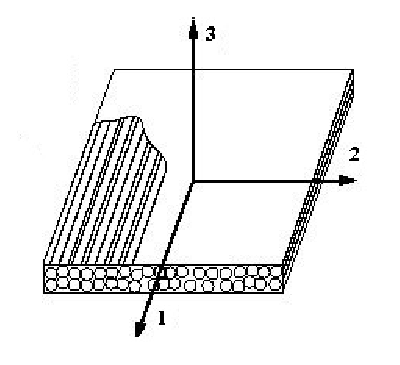
\includegraphics{Direcciones}
% figure caption is below the figure
\caption{ Directions in the laminate \cite{imagen}}
\label{fig:1}       % Give a unique label
\end{figure}
%\vspace{-1cm}
There are three failure modes for interlaminar fracture: Mode I (opening), mode II (shearing) and mode III (tearing). The theoretical modeling of delamination in composite materials can be made according to Linear-Elastic Fracture Mechanics . Each mode has an associated value of fracture toughness: $G_I_C, G_I_I_C, G_I_I_I_C$ defined as the energy available for the advance of crack per unit area or Energy Release Rate.\\

Fracture Toughness can be defined as:
\begin{equation}
G=\frac{P^2}{2\cdot t_c} \frac{\partial C}{\partial a}
\end{equation}

Where, $P$ is the load, $C$ is the compliance which corresponds to the inverse of the stiffness or inverse of the slope of the load - displacement curve, $t_c$ the thickness and a denotes the length of delamination.\\ 

The tensile test consists in subjecting the specimen to a tensile load along its main axis, causing an elongation of the specimen in that direction until it reaches the break point. In the  shear plane test, a tensile test is performed on a laminate $[\pm 45^\circ]$ locating two strain gages, one in longitudinal direction and another one in transverse direction \cite{miravete}.\\

The most common used test to evaluate the interlaminar fracture toughness in mode I is Double Cantilever Beam, where opening forces are applied on the specimen by means of hinges or tabs attached to one end of the specimen. In the test Mixed Mode I / II, an apparatus that splits the load into two: one of them is applied via tabs located at the ends of the delaminated section of the specimen, and the other is applied via rollers which rest against the region not delaminated.\\ 

The failure criteria are intended to predict the failure of the sheet. Following the approach used in this paper is exposed.\\ 

Theory of maximum deformation: The failure occurs when any component of strain along the principal axes of the material exceeds or equals the experimental strain value to which the failure occurs and one of the following equations are true \cite{arias}:
\begin{equation}
$\varepsilon_1=\varepsilon_1_t^u,$   si   $\varepsilon_1>0$   {\'o}   $|\varepsilon_1|=\varepsilon_1_c^u,$   si   $\varepsilon_1<0$\\
\end{equation}
\begin{equation}
$\varepsilon_2=\varepsilon_2_t^u,$   si   $\varepsilon_2>0$   {\'o}   $|\varepsilon_2|=\varepsilon_2_c^u,$   si   $\varepsilon_2<0$\\
\end{equation}
\begin{equation}
$$|\gamma_4|$$=$\gamma_4^u,$   $|\gamma_5|$=$\gamma_5^u,$      $|\gamma_6|$$=$$\gamma_6^u,$

\end{equation}\\

Where , $\varepsilon_1, \varepsilon_2$ represent the normal strain and $\gamma_4, \gamma_5,$\\ $\gamma_6$ shear strains in the point of interest; $c, t$, indicate compressive and tensile respectively,  these should be always positive.\\

A wind turbine is a device which uses the power of the wind passing through its blades to cause a moment that moves the rotor shaft, transforming kinetic energy into electricity. The horizontal axis turbines are facing the wind and its axis of rotation is parallel to the ground. The energy obtained in a wind turbine is determined by the energy of the wind passing through the rotor, which depends on the air density, wind speed and swept area by the blades \cite{calvo}.


\vspace{-0.5cm}
%\subsection{Subsection title}
\section{State of the art}
\label{sec:2}
Some researchers have developed methods for aerodynamic and power analysis of wind turbines. In a NREL (National Renewable Energy Laboratory) technical report, the geometry of a conventional wind turbine and the results obtained when tested in the wind tunnel \cite{nrel} is presented; these values are then used as reference by Sorensen et al for comparison with those resulting from Computational Fluid Dynamics analysis and demonstrates the capacity of the software tool \cite{sor}. Also, Lawson et al, presented a methodology for aerodynamic simulation where meshing characteristics and control volume adequate for analysis are discussed in more depth \cite{lawson}.\\

A research performed by C{\'a}rdenas et al, presents the numerical validation of Thin-Walled Beam model with finite elements for a wind turbine blade. One of the most advanced formulations which are achieved coupling effects of non-linearity, arbitrary cross sections and anisotropic material, is the Variational Asymptotic Beam Sectional Analysis, which provides good results of stress / strain on finite element validations of models in three dimensions \cite{cardenas}.\\

Vasjaliya and Gangadharan developed a Fluid Structure Interaction simulation of a wind turbine blade to optimize it. The aerodynamic results of the blade obtained are transferred to the structural analysis module to calculate the constraints, strains and stresses which are taken as output parameters to optimize the iterative process to achieve the best performance design \cite{vas}.\\

A model developed following an investigation by the University of Minnesota combines the finite element models in a shell and standard beam for structural analysis of a wind turbine blade. The beam model is simpler than the shell one and can be used to study the interaction between the blade and the fluid in order to identify the forces acting on the blade, instead, the shell model is more detailed as to the response of certain areas of the blade to the forces acting as buckling \cite{dong}.\\

The results of both analyzes can be used to optimize the design parameters of the blade and improve performance, while the output power  increases \cite{dahl}.
\vspace{-0.6cm}
\section{Mechanical Characterization}
\label{sec:3}
Four laminates are manufactured: Unidirectional $0^\circ$, Unidirectional $45^\circ$ , Woven $0^\circ$and Woven $45^\circ$. The technique used is Vacuum Bagging Hand Lay up, which uses air pressure to keep the resin in place during curing by optimizing the content of matrix and improving the interlaminar adhesion between layers \cite{west}.\\ 

Once laminates have been manufactured and are completely cured, the extraction of the samples for mechanical characterization test is made by water jet cutting. Dimensions of the specimens are taken from the standards used for carrying out the tests: ASTM D638, D3518, D5528 and D6671.\\

Experimentally, the following physical properties were obtained: carbon / epoxy laminates density with unidirectional carbon fiber and woven as reinforcement: 1.3805 $g/cm^3$ and 1.374 $g/cm^3$; unidirectional carbon fiber, woven and epoxy resin density: 1.678 $g/cm^3$, 1.724 $g/cm^3$ and 1.138 $g/cm^3$; Weight of dry sheet of unidirectional carbon fiber and woven: 310.5 $g/m^2$ y 184.9 $g/m^2$; volume fraction of laminates with unidirectional carbon fiber and woven as reinforcement: 57{\%} and 49{\%}; Cured ply thickness with unidirectional carbon fiber and woven as reinforcement : 0.3 mm and 0.22 mm.\\

\begin{table,array}%[H]
% table caption is above the table
\caption{Table 1. Engineering constants obtained}  %Please write your table caption here}
\label{tab:1}       % Give a unique label
% For LaTeX tables use
\begin{center}
\begin{tabular}{ccc}
\hline\noalign{\smallskip}
Property & Unidirectional & Woven  \\
\hline\noalign{\smallskip}\hline\noalign{\smallskip}
$E_1$ $[GPa]$& 89.38 & 54.28 \\
$E_2$ $[GPa]$& 6.05 & 53.65 \\
$G_1_2$ $[GPa]$& 5.03 & 5.19 \\
$\upsilon_1_2$& 0.347 & 0.054\\
\noalign{\smallskip}\hline
\end{tabular}
\end{center}
\end{table,array}\\
\vspace{0.25cm}
Where\\
$E_1$: Young Modulus in longitudinal direction\\
$E_2$: Young Modulus in transverse direction\\
$G_1_2$: Shear Plane Modulus \\
$v_1_2$: Poisson Ratio\\

\begin{table,array}%[H]
% table caption is above the table
\caption{Table 2. Maximum Strength and Strain obtained}  %tests  %Please write your table caption here}
\label{tab:2}       % Give a unique label
% For LaTeX tables use
\begin{center}
\begin{tabular}{ccc}
\hline\noalign{\smallskip}
Property & Unidirectional & Woven  \\
\hline\noalign{\smallskip}\hline\noalign{\smallskip}
$\sigma_1_t^u$ $[MPa]$& 584.2 & 439.1 \\
$\sigma_2_t^u$ $[MPa]$& 17.9 & 529.6 \\
$\tau_1_2^u$ $[MPa]$& 31.9 & 51.48 \\
$\varepsilon_1_t^u$& 0.0065 & 0.0081\\
$\varepsilon_2_t^u$& 0.0030 & 0.0099\\
$\gamma_1_2^u$& 0.0063 & 0.0099\\
\noalign{\smallskip}\hline
\end{tabular}
\end{center}
\end{table,array}\\
\vspace{0.25cm}

Where\\
$\sigma_1_t^u$: Ultimate tensile strength in longitudinal direction\\
$\sigma_2_t^u$: Ultimate tensile strength in transverse direction\\
$\tau_1_2^u$: Ultimate shear plane strength\\
$\varepsilon_1_t^u$: Ultimate tensile strain in longitudinal direction\\
$\varepsilon_2_t^u$: Ultimate tensile strain in transverse direction\\
$\gamma_1_2^u$: Ultimate shear plane strain\\

\begin{table,array}%[H]
% table caption is above the table
\caption{Table 3. Interlaminar Fracture Toughness}  %Please write your table caption here}
\label{tab:3}       % Give a unique label
% For LaTeX tables use
%\resizebox{1cm}{3cm}{
\begin{center}
\begin{tabular}{ccccc}
\hline\noalign{\smallskip}
\multicolumn{5}{c}{DCB/MMB}\\
\hline
Sample & $G_I_I_C$ & $G_I_C$ & $G_I_I_C/G$ & $G$ \\
\hline\noalign{\smallskip}\hline\noalign{\smallskip}
DCB & --- & 366 & --- & ---  \\
MMB & 236.2 & 650.4 & 0.29 & 916.4 \\
\noalign{\smallskip}\hline
\end{tabular}
\end{center}%}
\end{table,array}\\
The units in the Table \ref{tab:3} are given in $[J/m^2]$.\\

Where\\
$G$: Mixed Mode I/II\\
$G_I_C$: Interlaminar Fracture Toughness in Mode I\\
$G_I_I_C$: Interlaminar Fracture Toughness in Mode II\\
$G_I_I_C/G$:Obtained Mixed Mode I/II\\

Obtained errors are presented in Table \ref{tab:4} and \ref{tab:5}. Characterized properties were compared with previuos works with different conditions to the ones achieved. However it would have been ideal to find values obtained under the same manufacture and testing conditions. \\

\begin{table,array}%[H]
% table caption is above the table
\caption{Table 4. Error Percentages (Unidirectional carbon fiber) \cite{pcl} \cite{navarro}  }  %tests  %Please write your table caption here}
\label{tab:4}       % Give a unique label
% For LaTeX tables use
\begin{center}
\begin{tabular}{cccc}
\hline\noalign{\smallskip}
Property & Experimental & Theorical & {\%}Error  \\
\hline\noalign{\smallskip}\hline\noalign{\smallskip}
$E_1$ $[GPa]$& 89.38 & 109 & 18 \\
$E_2$ $[GPa]$& 6.05 & 8.82 & 31.40 \\
$G_1_2$ $[GPa]$& 5.03 & 5 & 0.60 \\
$\upsilon_1_2$& 0.347 & 0.342 & 1.46\\
$\sigma_1_t^u$ $[MPa]$& 584.2 & 585.24 & 0.18\\
$\sigma_2_t^u$ $[MPa]$& 17.9 & 42 & 57.38 \\
$\tau_1_2^u$ $[MPa]$& 31.9 & 70 & 54.43\\
$\varepsilon_1_t^u$& 0.0065 & 0.0105 & 38.09\\
$\varepsilon_2_t^u$& 0.0030 & 0.0050 & 40.00\\
$\gamma_1_2^u$& 0.0063 & 0.0140 & 55.00\\
\noalign{\smallskip}\hline
\end{tabular}
\end{center}
\end{table,array}\\
\\
\vspace{4cm}
\begin{table,array}%[H]
% table caption is above the table
\caption{Table 5. Error Percentages (Woven) \cite{pcl} \cite{navarro}}  %tests  %Please write your table caption here}
\label{tab:5}       % Give a unique label\cite{pcl} \cite{navarro}
% For LaTeX tables use
\begin{center}
\begin{tabular}{cccc}
\hline\noalign{\smallskip}
Property & Experimental & Theorical & {\%}Error  \\
\hline\noalign{\smallskip}\hline\noalign{\smallskip}
$E_1$ $[GPa]$& 54.28 & 70 & 22.45 \\
$E_2$ $[GPa]$& 53.65 & 70 & 23.36 \\
$G_1_2$ $[GPa]$& 5.19 & 5 & 3.80 \\
$\upsilon_1_2$& 0.054 & 0.010 & 46.00\\
$\sigma_1_t^u$ $[MPa]$& 439.1 & 414.81 & 5.85\\
$\sigma_2_t^u$ $[MPa]$& 529.6 & 600 & 11.73 \\
$\tau_1_2^u$ $[MPa]$& 51.48 & 90 & 42.80\\
$\varepsilon_1_t^u$& 0.0081 & 0.0085 & 4.71\\
$\varepsilon_2_t^u$& 0.0099 & 0.0085 & 16.47\\
$\gamma_1_2^u$& 0.0099 & 0.0180 & 45.00\\
\noalign{\smallskip}\hline
\end{tabular}
\end{center}
\end{table,array}\\
 \\
\vspace{0.5cm}
\begin{table,array}%[H]
% table caption is above the table
\caption{Table 6. Error Percentages (Fracture Toughness) \cite{zu} }  %Please write your table caption here}
\label{tab:6}       % Give a unique label
% For LaTeX tables use
\begin{center}
%\resizebox{\textwidth}{!}{
%\scalebox{0.1}{1}{
\begin{tabular}{cccc}
\hline\noalign{\smallskip}
%\multicolumn{5}{c}{DCB/MMB}\\
%\hline
Property & Experimental & Theoretical & {\%}Error \\
\hline\noalign{\smallskip}\hline\noalign{\smallskip}
$G_I_C$  & 366 & 270.4 & 35.3  \\
$G_I_C$  & 236.2 & 161 & 46.7 \\
$G_I__I_C$  & 650.4 & 545 & 16.2\\
$G$  & 916.4 & 706 & 22.9\\
\noalign{\smallskip}\hline
\end{tabular}%}
\end{center}%}
\end{table,array}
\\
The properties values in the Table \ref{tab:6} are given in $[J/m^2]$, the first value corresponds to DCB value and the other ones to MMB values.
%\vspace{-0.7}
\section{Aerodynamic Simulation}
\label{sec:4}
\subsection{Numerical Validation}

A numerical simulation is performed to find the aerodynamic loads of the wind turbine blade NREL phase VI. The results are then compared with the known experimental values of the wind turbine, scale tested in a wind tunnel at NASA Ames Research Center.\\

 In order to generate the moving reference frame (required to simulate the angular velocity of the rotor through the rotational movement of the surrounding flow), it should be constructed  an internal control volume containing the mesh elements surrounding the blade and the flow separation region and an external volume for external elements to the rotor \cite{lawson}. Where $R$ is the radius of the blade, the control volume where it is located has a radius of $1.5R$ and $10R$ length. The outer volume has a radius of $3R$ and $12R$ length in order to allow free flow development along the domain \cite{ijera}.\\

The mesh obtained has a skewness or maximum deformation element  ratio of  0.969 and 1.434.711 cells, enough to copy the whole shape of the geometry, as values found in previous studies where a similar number of elements is obtained in the mesh \cite{nata}.\\

The simulation is carried out under steady state and is based on pressure as it does not consider compressibility effects that generate changes in the density. For these conditions the governing equations of continuity and momentum are used. Calculations are performed using the model of turbulence $k-\omega$ Shear Stress Transport based on the transport equations for the turbulent kinetic energy. The solution method used is the Navier - Stokes.\\

NREL VI phase wind turbine blade is simulated at speeds 7, 10, 13, 15, 20 and 25 $m/s$, angular velocity between 71.9 RPM and 72.1 RPM, density 1225 $kg/m^3$ and 1.7894 $kg/m\cdot s$ The values obtained by the CFD simulation and experimental obtained by NREL by testing in the wind tunnel of the wind turbine, found in the article by Sørensen et al, are presented in Figure \ref{fig:2}.\\ 

Both curves in Figura \ref{fig:2} present a similar behavior and near values for each velocity, which indicates that obtained results are according the expected.  

\begin{figure}[H]
% Use the relevant command to insert your figure file.
% For example, with the graphicx package use
  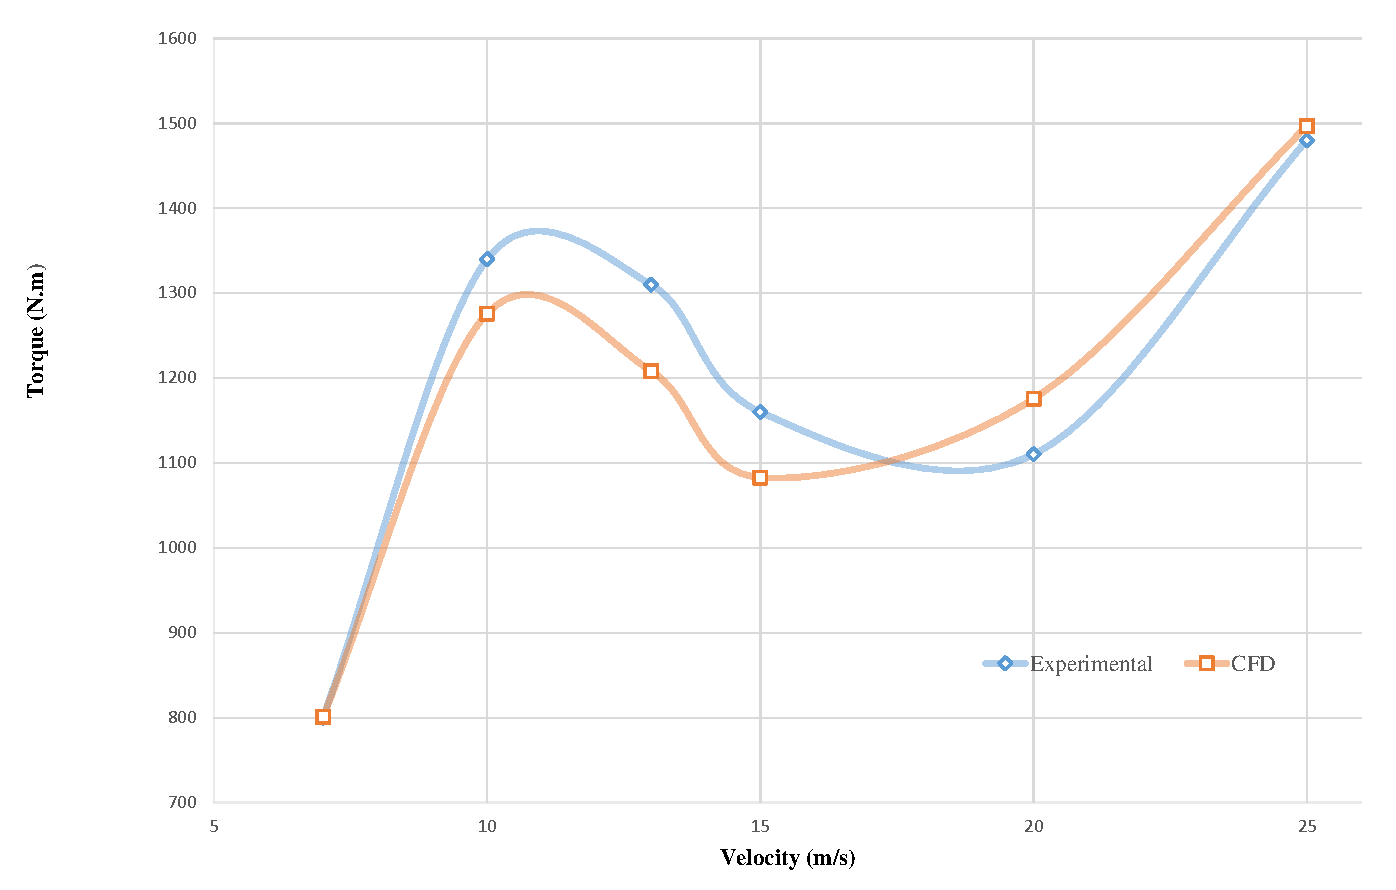
\includegraphics[width=0.5\textwidth]{vali}%antesde{}
% figure caption is below the figure
\caption{Comparative graph between the values obtained in CFD and experimental.}
\label{fig:2}       % Give a unique label
\end{figure}

\subsection{Aerodynamic simulation of bioinspired wind turbine blade}

The aerodynamic simulation was performed based on the validated model. A blade of the bio-inspired wind turbine was simulated in CFD, taking the geometry designed within the research project "Development of functional prototype for technical and commercial evaluation of small-scale bio-inspired wind turbine" by GIIA (Aerospace Engineering Research Group), following the same parameters for the volume control construction and simplifications in the validated model. See Figure \ref{fig:3}.

\begin{figure}[H]
% Use the relevant command to insert your figure file.
% For example, with the graphicx package use
  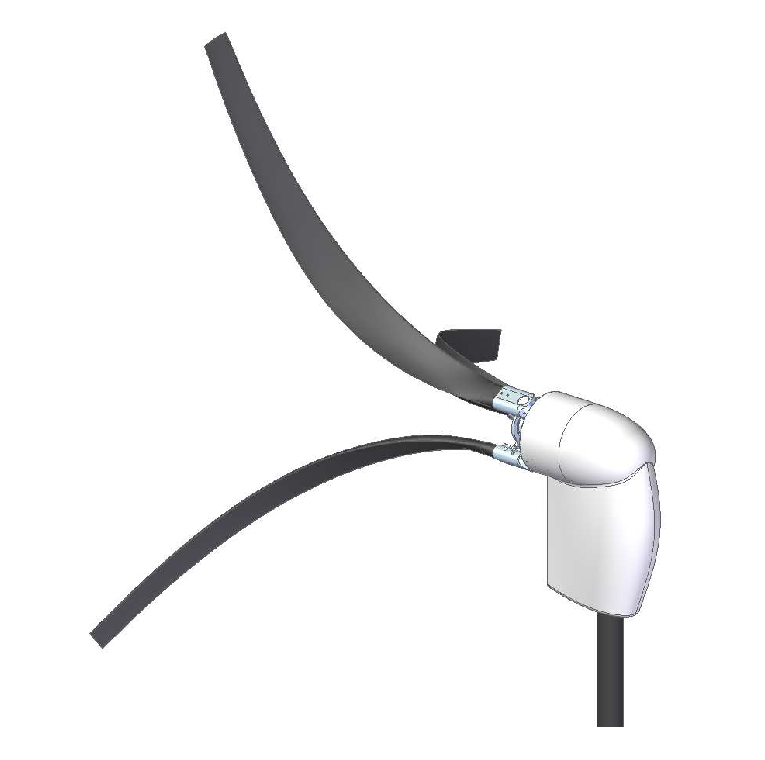
\includegraphics[width=0.2\textwidth]{Rotor}%[width=0.45\textwidth]antesde{}
% figure caption is below the figure
\caption{Bioinspired Wind Turbine}
\label{fig:3}       % Give a unique label
\end{figure}
\vspace{-0.3cm}
After ensuring meshing quality similar to that obtained in the validation,  the blade is simulated with a wind speed of 13 $m/s$, angular speed 43 $rad/s$, air density 1.225 $g/cm^3$ and pressure 101325 $Pa$. Using the same validation turbulence model, a torque of 35.904 $N\cdot m$ for each blade corresponding to a total rotor power of 4.632 $KW$ is obtained.

\begin{equation}
P_r = n_r\cdot \tau\cdot \omega
\end{equation}
Where $P_r$ is the rotor power,  $n_r$ the number of blades,  $\tau$ is one blade’s torque and, $\omega$ the angular velocity to which the wind turbine operates. \\ 

In the figures \ref{fig:4} to \ref{fig:7}, the pressure distribution is observed around the blade profile in four different sections. It can be clearly seen that at the root and $r/R= 0.5$ blade section, the stagnation point of the profile, where speed is zero and thus the pressure is high, it is above the leading edge due to negative attack angle to which it is encountered.

\begin{figure}[H]
% Use the relevant command to insert your figure file.
% For example, with the graphicx package use
  \includegraphics[width=0.45\textwidth]{fig1}
% figure caption is below the figure
\caption{Pressure contour of the blade profile in $r/R=0.25$}
\label{fig:4}       % Give a unique label
\end{figure}

\begin{figure}[H]
% Use the relevant command to insert your figure file.
% For example, with the graphicx package use
  \includegraphics[width=0.45\textwidth]{fig2}
% figure caption is below the figure
\caption{Pressure contour of the blade profile in $r/R=0.5$}
\label{fig:5}       % Give a unique label
\end{figure}
\vspace{-0.6cm}
\begin{figure}[H]
% Use the relevant command to insert your figure file.
% For example, with the graphicx package use
  \includegraphics[width=0.45\textwidth]{fig3}
% figure caption is below the figure
\caption{Pressure contour of the blade profile in $r/R=0.75$}
\label{fig:6}       % Give a unique label
\end{figure}
\vspace{-0.6cm}
\begin{figure}[H]
% Use the relevant command to insert your figure file.
% For example, with the graphicx package use
  \includegraphics[width=0.45\textwidth]{fig4}
% figure caption is below the figure
\caption{Pressure contour of the blade profile in $r/R=0.94$}
\label{fig:7}       % Give a unique label
\end{figure}

The pressure differences between the upper surface and inner of the blade, indicates a lift generation on those zones and that there is no profile loss presence despite the angle is relative to the wind, due to the curvature of the geometry.\\

In later sections, from $r / R = 0.75$ to the blade tip, normal behavior of the pressures on the profiles is observed so that the lift force is generated in all sections of the blade, although the pressure difference on the tip between the surface is smaller. Thus, all blade sections contribute to the generation of torque while the tip contributes minimally.\\

The pressure distribution profile obtained in this simulation is an input parameter in fluid-structure simulation, which is subsequently developed in order to make aerodynamic forces on the wind turbine match inertial forces.

\section{Fluid structure simulation of the bioinspired wind turbine blade}
\label{sec:5}

ANSYS  simulation comprises two modules’ coupling: Static Structural and ACP. The first is used to define the type of composite to be used including properties, stacking sequence and fiber orientation. While in the second one, the boundary conditions of the problem are established, the loads are imported from the module Fluent and the effect of the interaction between the aerodynamic and inertial loads is evaluated.\\

Woven and unidirectional carbon fiber are used. Linear elastic behavior for orthotropic material is set and orthotropic elasticity, strain and strength limits are defined. The input mechanical properties required by the software are elasticity modulus, Poisson's ratios, shear modules, tensile, compression and shear strength and strain limits. Some of these properties were previously characterized and presented in Table \ref{tab:1}. Others are assumed or consulted.\\
 
A shell mesh is obtained, consisting of triangular and tetrahedral elements in the body, and the orthogonal type elements in the edge. It has a skewness of 0.830 and 3574 elements. In the structural analysis of the blade, boundary conditions must be defined to restrict the degrees of freedom (in both rotation and translation) and adequately simulate their coupling to the hub. Fixed Support tool is used and it is associated to the cylindrical surface that forms the root. An angular velocity of 43 $rad / s$ around axis z is set to the body. The pressure distribution profile is imported to the structural module by pairing it with Fluent.\\

The assignment of the material is not uniform throughout the blade, due to the thickness not being constant along the geometry, but decreasing as it approaches the tip; also some areas are subjected to greater stress than others, so they must have greater thickness to withstand the loads properly. This discrimination is achieved by splitting the geometry into regions, considering distribution of local deformations. See Figure \ref{fig:8}.

\begin{figure}[H]
% Use the relevant command to insert your figure file.
% For example, with the graphicx package use
  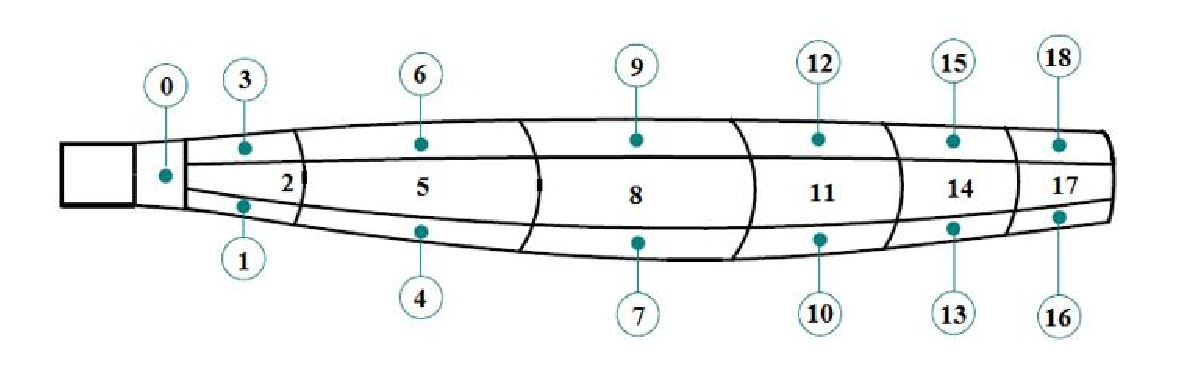
\includegraphics[width=0.45\textwidth]{p1}
% figure caption is below the figure
\caption{Geometry split into regions }
\label{fig:8}       % Give a unique label
\end{figure}
\vspace{-0.7cm}
The iterative design process had as main criterion the balance between aerodynamic performance and structural integrity. Aerodynamic loads act opposite to the inertial loads, formed by the effect of the rotational inertia influenced significantly by the weight. The stresses and strains produced by the aerodynamic phenomenon counter with inertial effects, being these predominant for the solution of the problem.\\

The chosen analysis criterion is based on the observation of total strains in the blade instead of stress. This is because with strains, it was possible to visualize more clearly the critical zones of the blade, where greater thickness is required, and additionally it was possible to determine which type of fiber was recommended for each region.\\

After adjusting the thickness and laminates and simulating real operating conditions, nominal displacement of 31.1 mm was obtained, fulfilling one of the restrictions previously imposed on the aerodynamic design of the blade. This restriction is that the displacement must not exceed a value of 50 mm, if it is above, the geometry gets deformed in a considerable way and aerodynamic performance of the blade can’t be guaranteed. In Figure \ref{fig:9} and \ref{fig:10} it can be observed the displacement suffered by the blade due to inertial loads. However this is relatively small compared with the overall size of the blade.


\begin{figure}[H]
% Use the relevant command to insert your figure file.
% For example, with the graphicx package use
  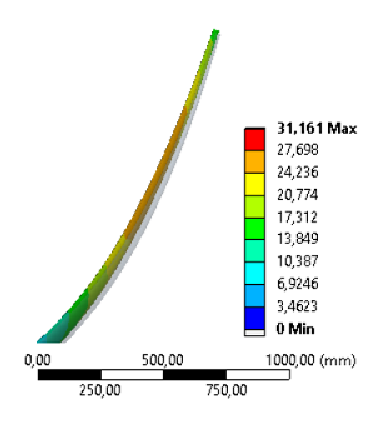
\includegraphics[width=0.3\textwidth]{p2}
% figure caption is below the figure
\caption{Total Deformation Contour. Blade side view. Angular speed 43 $rad/s$}
\label{fig:9}       % Give a unique label
\end{figure}

\begin{figure}[H]
% Use the relevant command to insert your figure file.
% For example, with the graphicx package use
  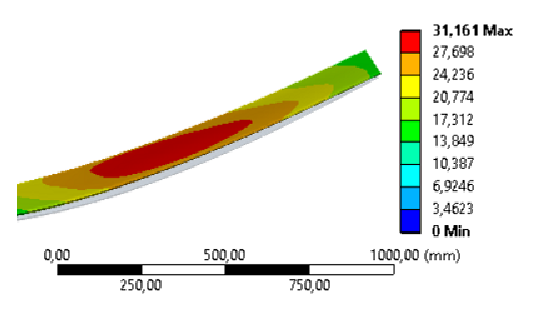
\includegraphics[width=0.4\textwidth]{p3}
% figure caption is below the figure
\caption{Zoom in blade tip. Original vs displaced geometry}
\label{fig:10}       % Give a unique label
\end{figure}
%\vspace{-1.0cm}
The tip is a high displacement area due to it is located away from the center of gravity and root. This effect is magnified with the unconventional shape of the blade; curvature affects the properties of inertia and increases the complexity of the problem. In Figure \ref{fig:11}, the red lines are drawn from the trailing edge to the leading edge for both geometries. The parallelism indicates that the profile displaces but does not rotate, that is, no torsion occurs as a result of the loads to which is subjected the blade, which means that the geometry is not modified and aerodynamic performance is not affected.
\vspace{-1.0cm}
\begin{figure}[H]
% Use the relevant command to insert your figure file.
% For example, with the graphicx package use
  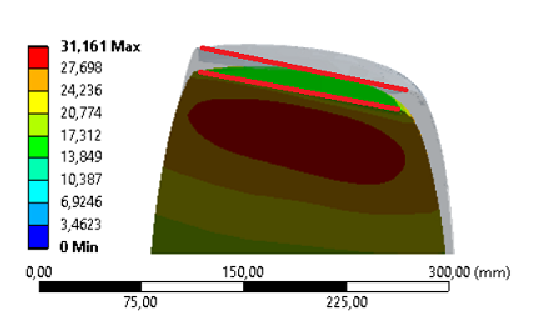
\includegraphics[width=0.4\textwidth]{p4}
% figure caption is below the figure
\caption{Tip profiles. Original vs displaced geometry}
\label{fig:11}       % Give a unique label
\end{figure}
Additionally, the maximum strain level was 2157 microstrains. This value is very low for a type of material like carbon fiber whose maximum tensile strain limits are around 6500 microstrains for unidirectional fiber and 8100 microstrains for woven, according to the properties characterized. While in shear it may reach a value of 6300 for unidirectional and 9900 for woven. See Figure \ref{fig:12} and Figure \ref{fig:13}.
\begin{figure}[H]
% Use the relevant command to insert your figure file.
% For example, with the graphicx package use
  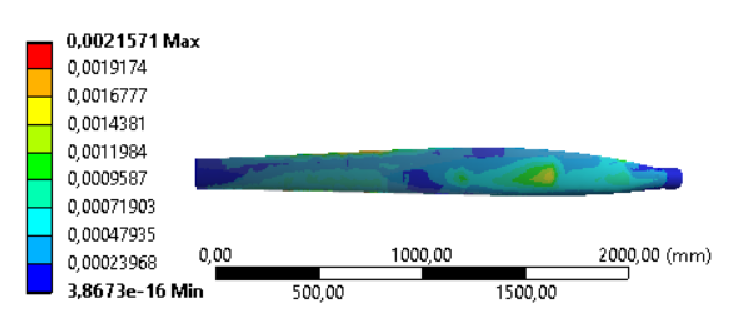
\includegraphics[width=0.45\textwidth]{p5}
% figure caption is below the figure
\caption{Total Strain Contours }
\label{fig:12}       % Give a unique label
\end{figure}

\begin{figure}[H]
% Use the relevant command to insert your figure file.
% For example, with the graphicx package use
  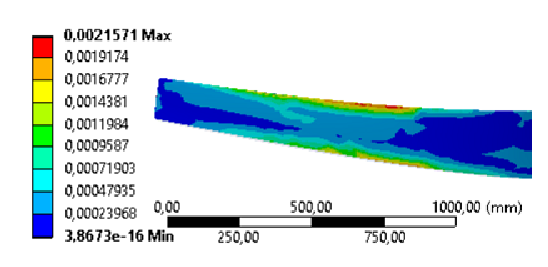
\includegraphics[width=0.45\textwidth]{p6}
% figure caption is below the figure
\caption{Total Strain Contours in region 15, inner Surface  }
\label{fig:13}       % Give a unique label
\end{figure}

Colombian Technical Standard ICONTEC "Wind Turbines: Design Requirements for Small Wind Turbines" indicates the safety factors for fatigue and failure analysis of wind turbines. For the case study, an aeroelastic model with design data (angular speed and power) is used. Therefore, the safety factor to be guaranteed is at least 1.35 (ICONTEC 2009). The most critical value of microstrains of the characterized material is 6300 (unidirectional fiber under shear loads). The safety factor obtained is 2.92, which doubles the restriction imposed by the standard. The calculation of the safety factor obtained is shown.

%as required. Don't forget to give each section
%and subsection a unique label (see Sect.~\ref{sec:1}).
%\paragraph{Paragraph headings} Use paragraph headings as needed.
\begin{equation}
Safety Factor= \frac{Critical Value}{Obtained Value} = \frac{6300}{2157} = 2.92%a^2+b^2=c^2
\end{equation}\\

Furthermore, it was essential to ensure that the laminates were symmetrical and balanced, because the terms of the stiffness matrix and the associated engineering constants coincide if the angle of orientation of the ply is $0^\circ$ or $90^\circ$. When the orientation angle is different from these values, a tensile-shear (torsion-bending) coupling is encountered, which decreases modules $E_1$ and $E_2$ \cite{miravete2}.\\

The 6 stacking sequences described below and shown in order of location from outside to inside were defined. See Figure \ref{fig:14} to \ref{fig:19}. 

\begin{figure}[H]
% Use the relevant command to insert your figure file.
% For example, with the graphicx package use
  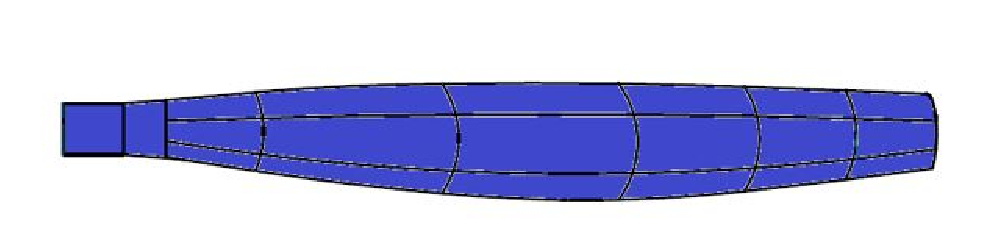
\includegraphics[width=0.45\textwidth]{p7}
% figure caption is below the figure
\caption{First stacking sequence  }
\label{fig:14}       % Give a unique label
\end{figure}
Sequence: [45  -45]\hspace{1cm}Thickness: 0.44 mm

\hspace{2cm}Weight: 0.632 Kg

\begin{figure}[H]
% Use the relevant command to insert your figure file.
% For example, with the graphicx package use
  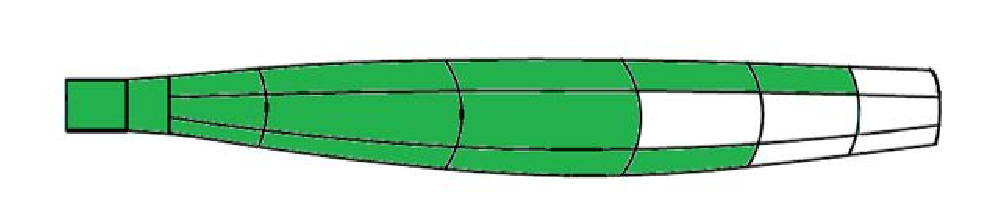
\includegraphics[width=0.45\textwidth]{p8}
% figure caption is below the figure
\caption{Second stacking sequence  }
\label{fig:15}       % Give a unique label
\end{figure}
Sequence: [45  -45]	\hspace{1cm}Thickness: 0.44 mm

\hspace{2cm}Weight: 0.394 Kg
\begin{figure}[H]
% Use the relevant command to insert your figure file.
% For example, with the graphicx package use
  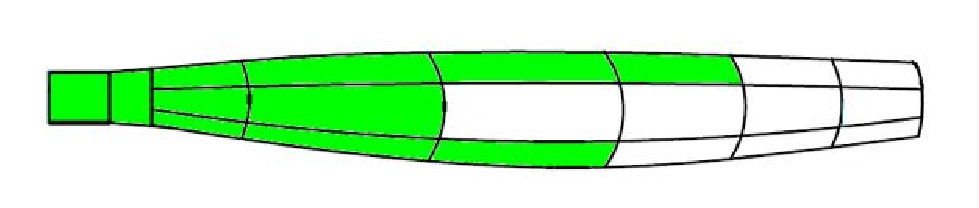
\includegraphics[width=0.45\textwidth]{p9}
% figure caption is below the figure
\caption{Third stacking sequence  }
\label{fig:16}       % Give a unique label
\end{figure}
Sequence: [0  90]_s	\hspace{1cm}Thickness: 0.88 mm 

\hspace{2cm}Weight: 0.540 Kg
\begin{figure}[H]
% Use the relevant command to insert your figure file.
% For example, with the graphicx package use
  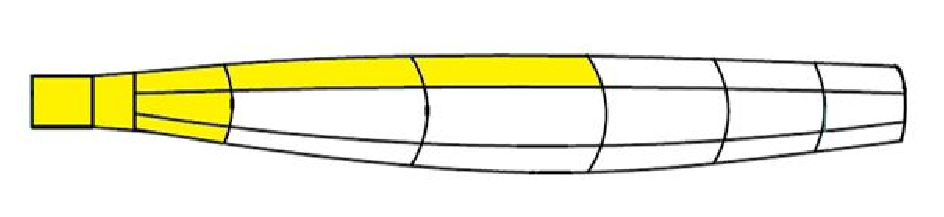
\includegraphics[width=0.45\textwidth]{p10}
% figure caption is below the figure
\caption{Fourth stacking sequence  }
\label{fig:17}       % Give a unique label
\end{figure}
Sequence: [0 0 0 45 -45]_s	\hspace{1cm}Thickness: 3.0 mm 

\hspace{2cm}Weight: 1.011 Kg
\begin{figure}[H]
% Use the relevant command to insert your figure file.
% For example, with the graphicx package use
  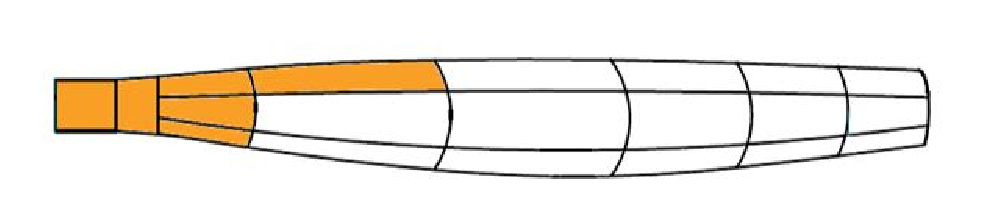
\includegraphics[width=0.45\textwidth]{p11}
% figure caption is below the figure
\caption{Fifth stacking sequence  }
\label{fig:18}       % Give a unique label
\end{figure}
Sequence: [0 0 0 45 -45]_s	\hspace{1cm}Thickness: 3.0 mm 

\hspace{2cm}Weight: 0.775 Kg
\begin{figure}[H]
% Use the relevant command to insert your figure file.
% For example, with the graphicx package use
  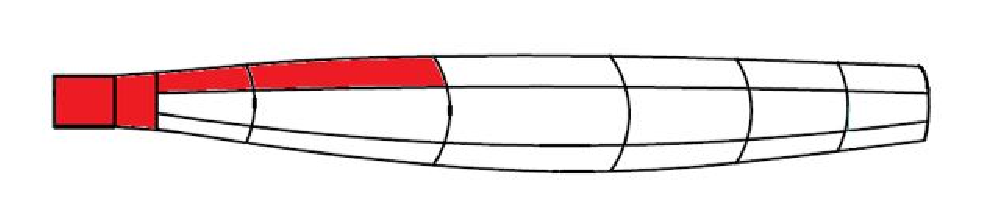
\includegraphics[width=0.45\textwidth]{p12}
% figure caption is below the figure
\caption{Sixth stacking sequence  }
\label{fig:19}       % Give a unique label
\end{figure}
Sequence: [45 -45]_s	\hspace{1cm}Thickness: 1.2 mm 

\hspace{2cm}Weight: 0.249 Kg\\

These stacking sequences were defined for outer Surface in the same way as the inner Surface. Total blade weight is 3.6 Kg, complying with design restrictions set, which required the minimum weight in order to reduce the inertia of the wind turbine. \\

The failure criterion used was the maximum strain, which allows to specify the strain limits for the material obtained in the characterization; as opposed to other criteria such as Tsai-Hill and Tsai-Wu, which employs coupling factors from values found in the state of the art. To measure the failure modes, the IRF (Inverse Reverse Factor), defined as the inverse of the failure margin is used. An IRF whose value is greater than 1 indicates failure. Due to low deformations and displacements obtained with numerical simulation, this analysis not fault zones occurred in the blade, as shown in Figure \ref{fig:20}.

\begin{figure}[H]
% Use the relevant command to insert your figure file.
% For example, with the graphicx package use
  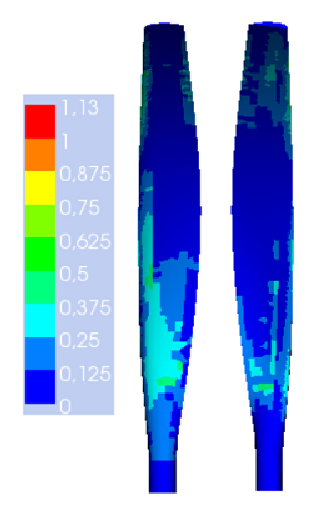
\includegraphics[width=0.25\textwidth]{p13}
% figure caption is below the figure
\caption{Results of maximum strain criterion }
\label{fig:20}       % Give a unique label
\end{figure}

\section{Conclusions}
\label{sec:6}
It is essential to control the fiber and resin content. If the last one is too low, the fibers are not adequately impregnated, and if too high, the volume fraction of reinforcement, responsible for the mechanical properties of the composite in tension, decreases.\\

The mechanical properties characterized allow to know the limit conditions to which the material may be subjected to define the structural design of the blade, where multidirectional stress are presented and which can be withstanded with variation of stacking sequences and type of carbon fiber used.\\

The cutting process has a significant impact on the mechanical characterization. It must be ensured that the central axis of the specimen matches the orientation of the fibers to be evaluated and that no stress concentration effects occur at the edges. Additionally, the extensometer to be used must be properly calibrated.\\

The error percentages of the properties characterized achieve average values of 29{\%} for unidirectional fiber and 22{\%} for woven. This is due to the aforementioned causes and that it was not found in literature properties obtained by vacuum assisted manual techniques but more complex methods and automated manufacturing, which reduces the possibility of defects in manufacturing.\\

It was shown that the methodology and validated aerodynamic model developed are valid and can be used in the aerodynamic simulation of the bio-inspired turbine because of the reliable results and acceptable errors $(\leq7{\%})$.\\

The pressure distribution profile obtained is adequate and representative of the pressures’ behavior acting on the blade, indicating a generation of forces and therefore torque, that demarcates the main function of the wind turbine. However, due to the geometry of the blade, there are sections where the attack angles are negative, and contributes minimum to torque generation.\\
 
A validation of the structural model was not performed due to unconventional shape of the blade. Nor it was possible to find a consolidated state of the art which provided a fluid structure model simulation applicable to the study case, or that evaluated the behavior of a wind turbine blade with the same materials characterized in this work. Therefore, an own model was built using knowledge acquired through software tutorials \cite{ansys}.\\

The most critical region, as observed in the numerical simulations FSI, is close to the inflection point, where a change of curvature creates high deflections in the geometry and constitutes as the displacement starting point.\\

The use of stacking sequences involving orientations at $0^\circ$, provides satisfactory characteristics of rigidity and strength in that direction. The plies oriented $\pm 45$ exhibit ideal mechanical properties when there are torsion problems, allowing to control the deformations generated by such forces.\\

A safety factor of 2.92 for bio-inspired wind turbine blade was obtained, more restrictive than the one imposed by ICONTEC, which ensures safe operation of the system and balances the errors obtained in the mechanical characterization.
% For one-column wide figures use
%\begin{figure}
% Use the relevant command to insert your figure file.
% For example, with the graphicx package use
%  \includegraphics{example.eps}
% figure caption is below the figure
%\caption{Please write your figure caption here}
%\label{fig:1}       % Give a unique label
%\end{figure}
%
% For two-column wide figures use
%\begin{figure*}
% Use the relevant command to insert your figure file.
% For example, with the graphicx package use
 % \includegraphics[width=0.75\textwidth]{example.eps}
% figure caption is below the figure
%\caption{Please write your figure caption here}
%\label{fig:2}       % Give a unique label
%\end{figure*}
%
% For tables use
%\begin{table}
% table caption is above the table
%\caption{Please write your table caption here}
%\label{tab:1}       % Give a unique label
% For LaTeX tables use
%\begin{tabular}{lll}
%\hline\noalign{\smallskip}
%first & second & third  \\
%\noalign{\smallskip}\hline\noalign{\smallskip}
%number & number & number \\
%number & number & number \\
%\noalign{\smallskip}\hline
%\end{tabular}
%\end{table}


%\begin{acknowledgements}
%If you'd like to thank anyone, place your comments here
%and remove the percent signs.
%\end{acknowledgements}

% BibTeX users please use one of
%\bibliographystyle{spbasic}      % basic style, author-year citations
\bibliographystyle{spmpsci}      % mathematics and physical sciences
%\bibliographystyle{spphys}       % APS-like style for physics
%\bibliography{biblio}   % name your BibTeX data base

% Non-BibTeX users please use
%\begin{thebibliography}{}
%
% and use \bibitem to create references. Consult the Instructions
% for authors for reference list style.
%
%\bibitem{RefJ}
% Format for Journal Reference
%Author, Article title, Journal, Volume, page numbers (year)
% Format for books
%\bibitem{RefB}
%Author, Book title, page numbers. Publisher, place (year)
% etc
%\end{thebibliography}
\bibliography{biblio}
\end{document}
% end of file template.tex

